\chapter{Optimizing Matrix Transpose}
\label{cha:optimizing_matrix_transpose}

\section{实验要求}
\label{sec2:shi_yan_yao_qiu_}

\par 在这一部分的实验中,需要实现cache友好的矩阵转置。矩阵转置是这样一种操作:对于一个矩阵$A$的转置$A^{T}$, $[A^{T}]_{ij} = [A]_{ji}$。在本实验中,将采用1KB直接映射,块大小为32bytes($E=1, C=1024, B=32$,$s=5, b=5$)的cache配置进行模拟以及测试。矩阵转置的目标是最小化cache miss次数。

\par 在实现时,对于矩阵转置程序做出如下限制:
\begin{itemize}
    \item 显示栈空间的使用:在转置函数中最多使用12个int类型的局部变量,而不能以任何其他形式使用额外的变量。
    \item 不能使用递归,如果使用辅助函数,则在任意时刻,从转置函数的栈帧到辅助函数的栈帧之间最多可以同时存在12个局部变量。
    \item 转置函数不能够改变矩阵A但是可以任意操作矩阵B。
    \item 不允许在代码中定义任何矩阵以及使用malloc及其变种。
\end{itemize}

\par 测试所使用的数据如下:
\begin{itemize}
    \item $32\times 32$的矩阵,cache miss次数小于300次得8分,大于60次得0分,处于中间的部分按照线性给分。
        $64\times 64$的矩阵,cache miss次数小于1300次得8分,大于2000次得0分,中间部分按照线性给分。
        $62\times 67$的矩阵,cache miss次数小于2000次得10分,大于3000次得0分,中间部分按照线性给分。
\end{itemize}

\section{实验设计}
\label{sec2:shi_yan_she_ji_}

\subsection{总体设计}
\label{sub2:zong_ti_she_ji_}

\par 在设计cache友好的转置之前,首先考虑普通的矩阵转置算法:
\inputCodeSetLanguage{c}
\begin{lstlisting}
void trans(int M, int N, int A[N][M], int B[M][N]) {
    int i, j;
    for (i = 0; i < N; ++i)
        for (j = 0; j < M; ++j)
            B[j][i] = A[i][j];
}
\end{lstlisting}
\par 这一函数的正确性毋庸置疑,但它并不是cache友好的,因为其并没有有效的利用cache。以$32\times 32$的矩阵为例,由于cache块大小为32bytes,也就是说一行能够存入8个整型变量,此时整个cache能够存入矩阵的8行。此时,如果同一个矩阵中同一列的两个整数相差了8行,那么先后访问这两个整数就会发生eviction。

\par 在上述平凡算法中,仅是在将矩阵的第一行转置的写入操作中就会发生24次cache eviction,而此后对于每一行的转置对应的B中的每一行的写入都会发生32次cache eviction,加上矩阵A和矩阵B同一行的冲突以及读取矩阵A时发生的冲突,一共会发生$32 + 32\times 32 + 32 + 24\times 4 = 1184$次cache miss,其中第一个32是首次读入矩阵A的前八行发生的cache miss,$32\times 32$是在将A的每一行存入B的每一列是发生的cache miss,第二个32是存取对角线元素时存入B导致A先前存入cache的部分发生cache miss,而最后的$24\times 4$则是读取A时每读取4行就会发生的24次cache miss。实际计算的结果如图\ref{fig:exampleCacheMiss}所示,这与计算的结果非常相近。

\begin{figure}[htb]
    \centering
    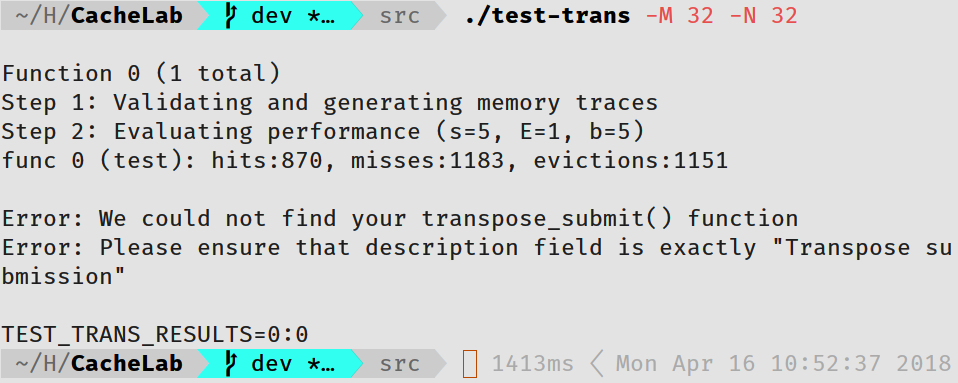
\includegraphics[width=0.8\linewidth]{exampleCacheMiss.png}
    \caption{普通转置运算cache miss结果}
    \label{fig:exampleCacheMiss}
\end{figure}

\par 为了减少实际的cache miss数,需要尽可能的利用时间局部性和空间局部性:
\begin{itemize}
    \item 时间局部性:尽可能的利用当前的cache block。
    \item 空间局部性:在尽可能小的范围内访问数据。
\end{itemize}
\par 此时,最容易想到的方法是矩阵分块和修改访问次序。就矩阵分块而言,需要考虑分块的大小,以便能够尽量高校地利用cache。由于本实验cache的大小是每行32字节,因此分块大小应为$8\times 8$,这样分块的每行就刚好能够存入cache的一行,从而有可能提高空间和时间的局部性。

\subsection{详细设计}
\label{sub2:xiang_xi_she_ji_}

\par 在$32\times 32$的矩阵中,如果读取或存放的两个数之间相差整数倍,则一定会发生一次cache miss,但在该矩阵转置的过程中,这对于对角线上的元素是不可能发生的。因此对于非对角线上的12个分块,读+写的cache miss数为$8\times 12 + 8\times 12 = 192$次,对于对角线上的分块读取A发生$8\times 4 = 32$次cache miss,B写入则发生$16\times 4 = 64$次cache miss,总共$192 + 32 + 64 = 288$次cache miss。这样就满足题目要求了。

\par 而对于$64\times 64$的矩阵而言,由于整个cache只能装下矩阵的前4行,经过初步计算后发现,如果使用与$32\times 32$的矩阵相同的方法,则对于每个分块转置需要cache miss次数为$8 + 8\times 8 = 72$次其中8次为读取A所发生的cache miss,而$8\times 8$次则是由于cache只能装下矩阵的4行而导致的B写入是发生的cache miss,于是转置所有分块会发生$64\times 72 = 4608$次cache miss。实际的初步实验结果为4611次,与理论结果相近,如图\ref{fig:exampleCacheMiss2}所示。

\begin{figure}[htb]
    \centering
    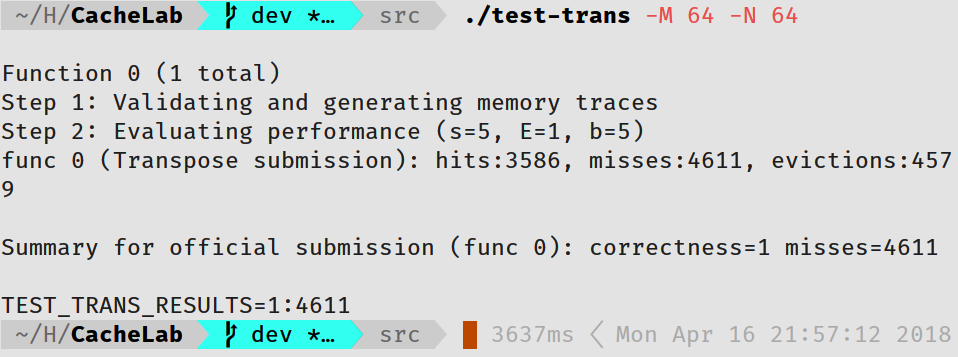
\includegraphics[width=0.8\linewidth]{exampleCacheMiss2.png}
    \caption{使用$8\times 8$分块转置$64\times 64$矩阵的cache miss数}
    \label{fig:exampleCacheMiss2}
\end{figure}

\par 由于主要的cache miss发生在存入B矩阵的过程中,而发生如此多的cache miss的原因是当矩阵变大后,cache只能存入矩阵的4行,因此推测如果使用$4\times 4$的分块应该能够减少cache miss次数。通过进一步的试验,发现如果使用$4\times 4$的分块,则cache miss的次数为1699次,如图\ref{fig:exampleCacheMiss3}所示。
\begin{figure}[htb]
    \centering
    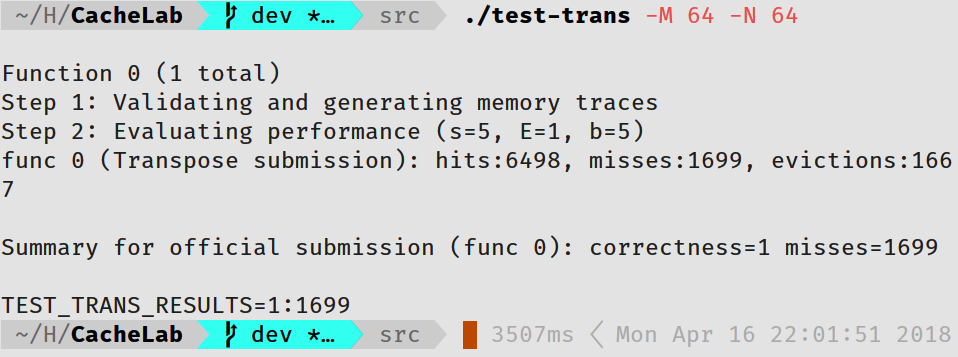
\includegraphics[width=0.8\linewidth]{exampleCacheMiss3.png}
    \caption{使用$4\times 4$分块转置$64\times 64$矩阵的cache miss数}
    \label{fig:exampleCacheMiss3}
\end{figure}

\par 虽然已经大大减小了cache miss的次数,然而依然不符合题目要求的1300次。其原因应该是使用$4\times 4$的矩阵不能够很好的利用全部的cache空间,每一次存取时cache line中一半的元素未能很好的被利用。
\par 为了能够更好的利用空进局部性,将B的一部分作为cache使用。依然使用$8\times 8$的分块,但在写入B矩阵时可以在满足cache不被替换的情况下首先将A的部分元素写入B的错误位置,然后在后续的操作中在考虑将其移至正确的位置。经过计算,采用如图\ref{fig:blockTrans}所示的策略进行对分块的转置效率较高。
\begin{figure}[htb]
    \centering
    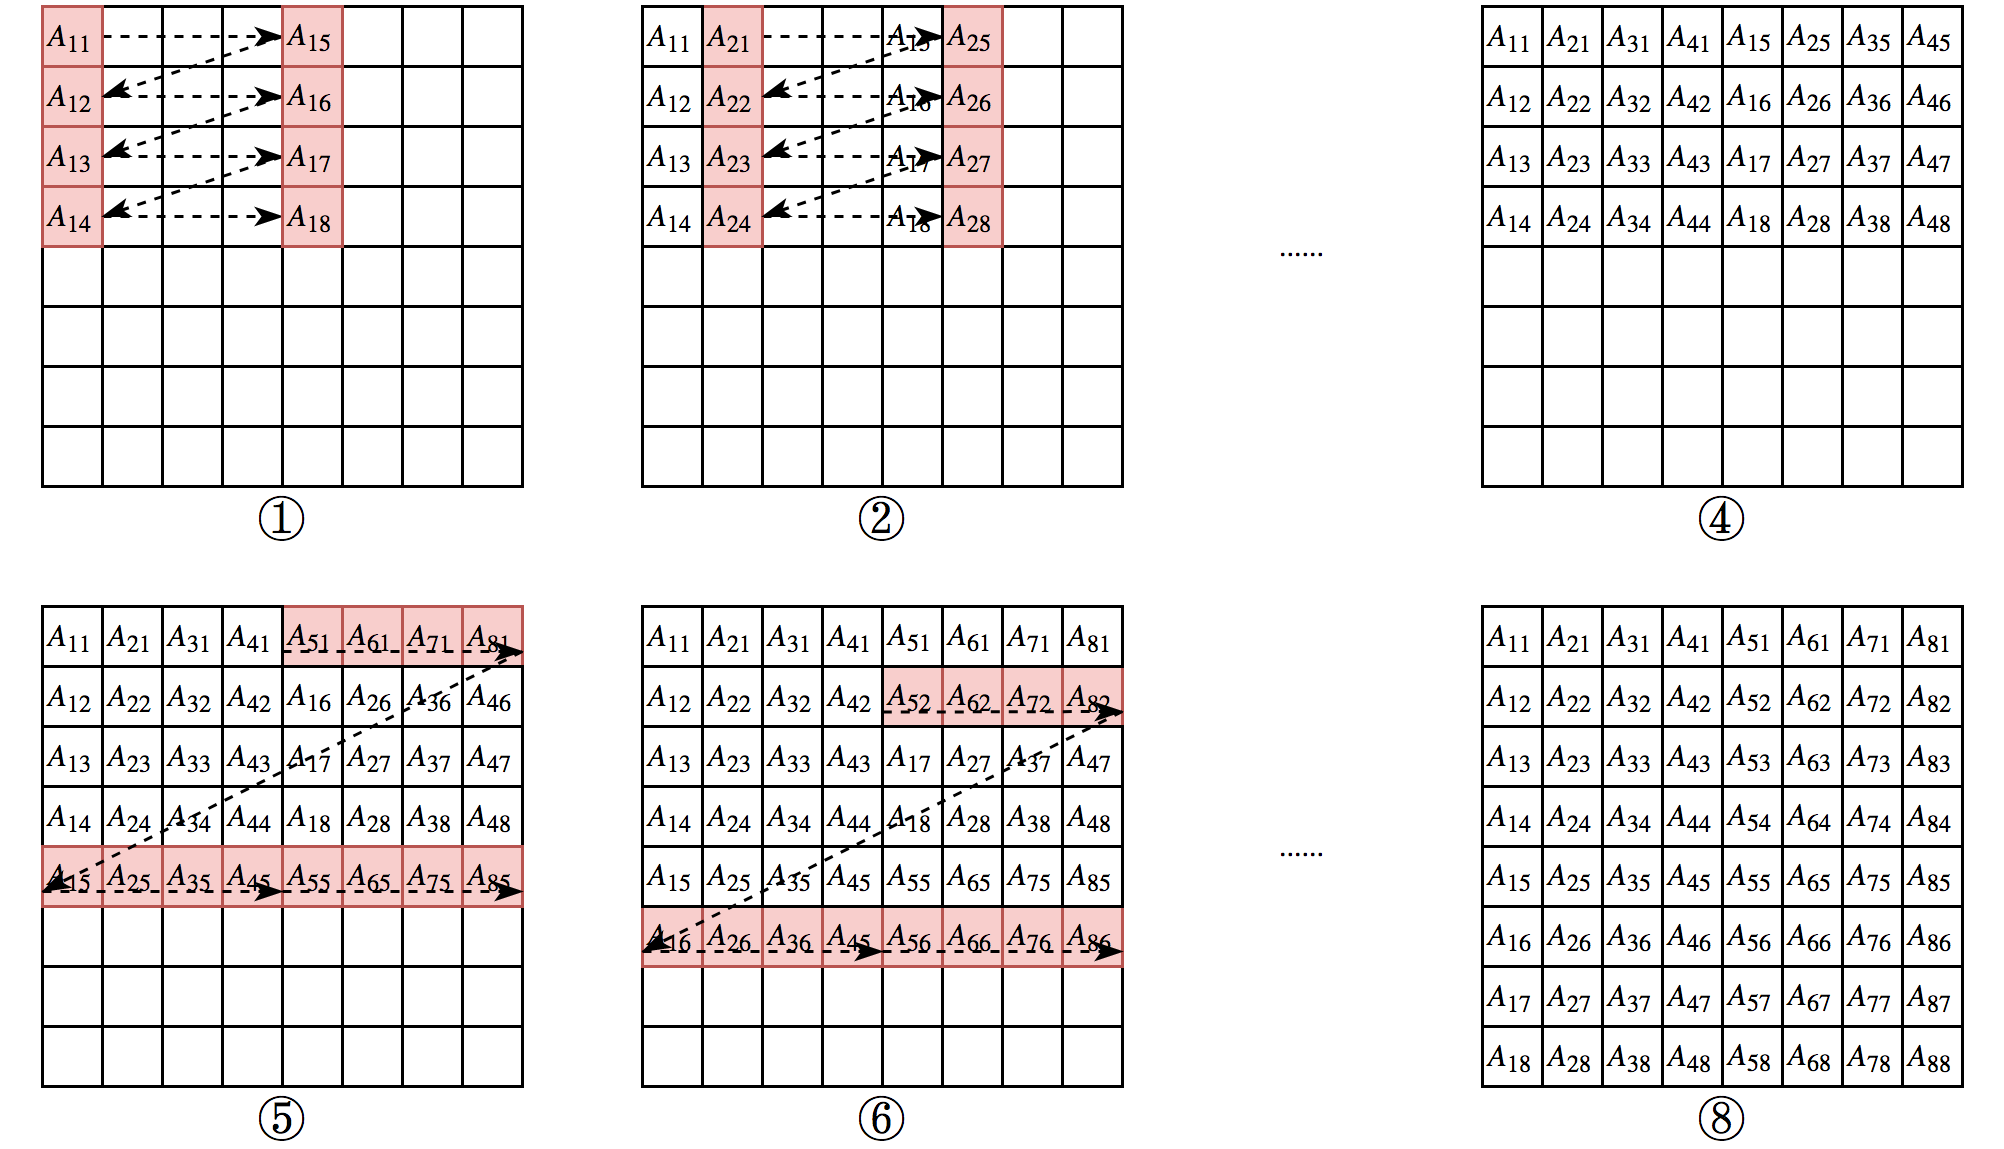
\includegraphics[width=0.95\linewidth]{blockTrans.png}
    \caption{分块转置策略}
    \label{fig:blockTrans}
\end{figure}

\par 图\ref{fig:blockTrans}表示对于B的写入过程,其中的阴影部分为当前步骤更新的元素,箭头表示更新的顺序。在步骤1中,读取A的第1行,并将前后部分分别填入$B_{11}\sim B_{41}$以及$B_{15}\sim B_{45}$的部分。此时为了减少cache miss,A第一行的后半部分被填入了错误的地方。接下来依次读入A的$2\sim 4$行并按照上述方法填入B对应的位置,这分别对应图\ref{fig:blockTrans}中的步骤$2\sim 4$。

\par 当步骤$1\sim 4$完成后,就进行较为复杂也较为重要的步骤。以第5步为例,使用8个局部变量中的4个存储$A_{51}\sim A_{81}$,并使用另外4个局部变量存储第1步存储到B中的$A_{15}\sim A_{45}$。然后,首先将$A_{51}\sim A_{81}$存储到$B_{15}\sim B_{18}$的位置,接下来将空出来的这4个局部变量用于存储$A_{55}\sim A_{85}$,最后将$A_{15}\sim A_{85}$存储到$B_{51}\sim B_{58}$的位置。这样,就同时完成了A分块中的右半部分的转置以及坐下部分的转置。

\par 使用这样的转置方法,对于每一个非对角块的转置而言,步骤$1\sim 4$中,除了第一步外,每一步对A的读取发生1次cache miss,对B的写入没有cache miss,而第一步对B的写入发生4次cache miss,一共$4 + 3\times 1 = 7$次。在步骤$5\sim 8$中,除了第5步外,读取A的一列4个元素发生不发生cache miss,而第5步发生4次。读取B的一行4个以及在同样的位置存入不发生cache miss。然后再次对于A的读取不发生cache miss(前面的读取已经缓存),然后对B写入8个元素发生1次cache miss。因此在步骤$5\sim 8$中,一共会发生$4 + 1 + 3\times 1 = 8$次。

\par 对于中心块的转置而言,在第$1\sim 4$以及$5\sim 8$步分别比非中心块多出4次和16次。因此对于整个矩阵的转置会发生$56\times (7 + 8) + 8\times (7 + 8 + 4 + 16) = 1120$次。这样,就能够满足题目要求了。

\par 对于$61\times 67$的矩阵,由于其条件比较宽松,预估使用普通分块即可达到要求。这一点将在接下来的章节中继续进行实验验证。

\section{实验过程}
\label{sec2:shi_yan_guo_cheng_}

\subsection{实验环境}
\label{sub2:shi_yan_huan_jing_}
实验环境同上章节\ref{sub:shi_yan_huan_jing_}。

\subsection{详细步骤}
\label{sub2:shi_yan_guo_cheng_}

\par 首先,处理$32\times 32$的矩阵。使用4个变量作为循环变量,进行分块转置后的代码如下:

\inputCodeSetLanguage{c}
\begin{lstlisting}
for (a = 0; a < N; a += 8)
     for (b = 0; b < M; b+=8)
         for(c = a; c < a + 8; ++c)
             for(d = b; d < b + 8; ++d)
                 B[d][c] = A[c][d];
\end{lstlisting}

\par 然而,经过测试后发现,发生了343次cache miss如图\ref{fig:cacheMiss1},未能达到题目要求。
\begin{figure}[htb]
    \centering
    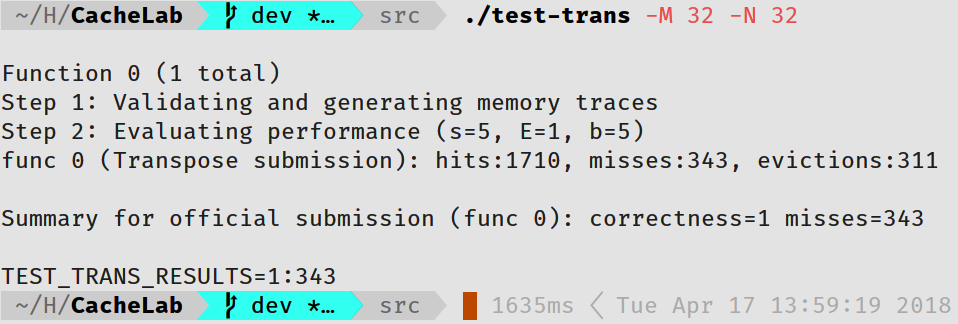
\includegraphics[width=0.8\linewidth]{cacheMiss1.png}
    \caption{首次对于$32\times 32$矩阵进行分块转置测试}
    \label{fig:cacheMiss1}
\end{figure}

\par 推测原因,是由于对角先访问的问题:由于A和B在内存中的位置是连续的,因此A和B的同一行被映射到了同一个cache line。此时进行对角线访问时一定会发生cache eviction。而由于A和B的元素是一个个处理的,因此会造成多次cache miss。要解决这一问题,需要一次性读入一整行。好在有12个局部变量可以使用,使用4个作为循环变量后还有8个可以用于存储临时值。修改后的代码如下:

\begin{lstlisting}
for (a = 0; a < N; a += 8) {
    for (b = 0; b < M; b += 8) {
        for (c = a; c < a + 8; ++c) {
            reg0 = A[c][b + 0]; reg1 = A[c][b + 1];
            reg2 = A[c][b + 2]; reg3 = A[c][b + 3];
            reg4 = A[c][b + 4]; reg5 = A[c][b + 5];
            reg6 = A[c][b + 6]; reg7 = A[c][b + 7];
            B[b + 0][c] = reg0; B[b + 1][c] = reg1;
            B[b + 2][c] = reg2; B[b + 3][c] = reg3;
            B[b + 4][c] = reg4; B[b + 5][c] = reg5;
            B[b + 6][c] = reg6; B[b + 7][c] = reg7;
        }
    }
}
\end{lstlisting}

\par 对于上述代码重新进行编译并测试,结果如图\ref{fig:cacheMiss2}所示,共287次cache miss,达到题目要求,且与计算结果几乎一致。
\begin{figure}[htb]
    \centering
    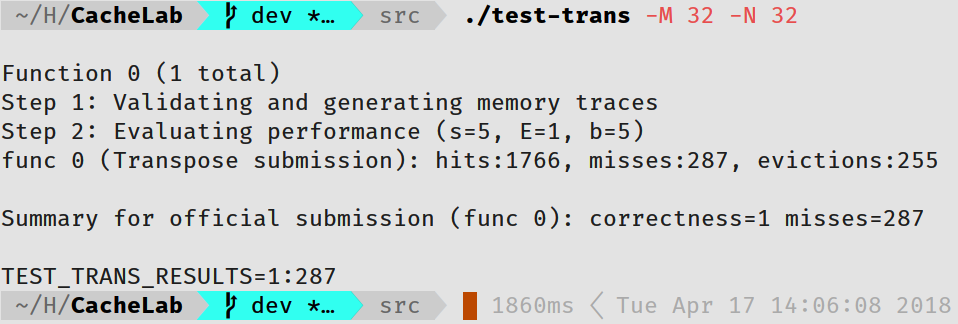
\includegraphics[width=0.8\linewidth]{cacheMiss2.png}
    \caption{对于修改后的代码进行测试}
    \label{fig:cacheMiss2}
\end{figure}

\par 接下来按照详细设计中的转置策略对于$64\times 64$的代码进行矩阵转置测试:
\begin{lstlisting}
for (a = 0; a < N; a += 8) {
    for (b = 0; b < M; b += 8) {
        for (c = a; c < a + 4; ++c) {
            reg0 = A[c][b + 0]; reg1 = A[c][b + 1];
            reg2 = A[c][b + 2]; reg3 = A[c][b + 3];
            reg4 = A[c][b + 4]; reg5 = A[c][b + 5];
            reg6 = A[c][b + 6]; reg7 = A[c][b + 7];
            B[b + 0][c] = reg0; B[b + 0][c + 4] = reg4;
            B[b + 1][c] = reg1; B[b + 1][c + 4] = reg5;
            B[b + 2][c] = reg2; B[b + 2][c + 4] = reg6;
            B[b + 3][c] = reg3; B[b + 3][c + 4] = reg7;
        }
        for (c = 0; c < 4; ++c) {
            reg0 = A[a + 4][b + c]; reg1 = A[a + 5][b + c];
            reg2 = A[a + 6][b + c]; reg3 = A[a + 7][b + c];
            reg4 = B[b + c][a + 4]; reg5 = B[b + c][a + 5];
            reg6 = B[b + c][a + 6]; reg7 = B[b + c][a + 7];
            B[b + c][a + 4] = reg0; B[b + c][a + 5] = reg1;
            B[b + c][a + 6] = reg2; B[b + c][a + 7] = reg3;
            reg0 = A[a + 4][b + c + 4]; reg1 = A[a + 5][b + c + 4];
            reg2 = A[a + 6][b + c + 4]; reg3 = A[a + 7][b + c + 4];
            B[b + c + 4][a + 0] = reg4; B[b + c + 4][a + 4] = reg0;
            B[b + c + 4][a + 1] = reg5; B[b + c + 4][a + 5] = reg1;
            B[b + c + 4][a + 2] = reg6; B[b + c + 4][a + 6] = reg2;
            B[b + c + 4][a + 3] = reg7; B[b + c + 4][a + 7] = reg3;
        }
    }
}
\end{lstlisting}
\par 上述代码中,\lstinline{for (c = a; c < a + 4; ++c)}循环内执行的代码对应图\ref{fig:blockTrans}策略中的第$1\sim 4$步,而\lstinline{for (c = 4; c < 4; ++c)}中执行的代码则对应图\ref{fig:blockTrans}策略中的第$5\sim 8$步。

\par 下面对于上述代码进行测试。运行Make进行编译后,执行./test-trans -M 64 -N 64进行测试,结果如图\ref{fig:cacheMiss3}所示。
\begin{figure}[htb]
    \centering
    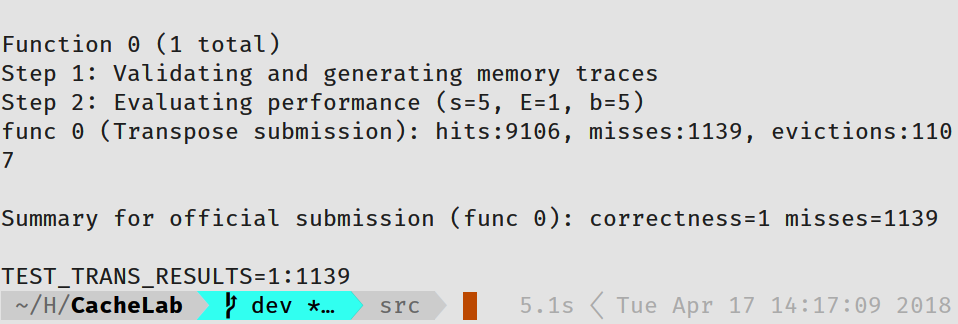
\includegraphics[width=0.8\linewidth]{cacheMiss3.png}
    \caption{$64\times 64$矩阵分块转置测试}
    \label{fig:cacheMiss3}
\end{figure}

\par 从图中可以看出,cache miss的次数为1139次,满足题目要求。

\par 对于$61\times 67$的矩阵,其策略也是使用分块来优化cache读写。然而61和67均为质数,无法找到一个明显的规律看出多少间隔能够填满一个cache。但由于要求比较宽松,因此无需考虑对角线处理,直接使用普通分块操作进行尝试。最后发现,$23\times 23$的分块能够满足要求,其代码如下:
\begin{lstlisting}
for (a = 0; a < N; a += 23)
    for (b = 0;  b < M; b += 23)
        for (c = a; c < a + 23 && c < N; ++c)
            for (d = b; d < b + 23 && d < M; ++d)
                B[d][c] = A[c][d];
\end{lstlisting}

\par 测试的结果如图\ref{fig:cacheMiss4}所示,共发生了1928次cache miss,小于要求的2000次。
\begin{figure}[htb]
    \centering
    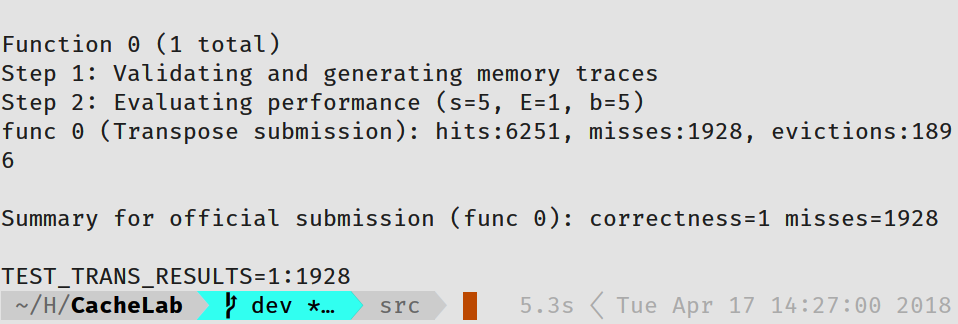
\includegraphics[width=0.8\linewidth]{cacheMiss4.png}
    \caption{$61\times 67$矩阵分块转置测试}
    \label{fig:cacheMiss4}
\end{figure}

\subsection{测试与分析}
\label{sub2:ce_shi_yu_fen_xi_}
\par 在完成了上述代码后,将所有代码整合进transpose\_submit函数中,然后在registerFunctions函数中注册transpose\_submit函数。整合后的函数如下:
\begin{lstlisting}
void transpose_submit(int M, int N, int A[N][M], int B[M][N]) {
    int a, b, c, d;
    int reg0, reg1, reg2, reg3, reg4, reg5, reg6, reg7;
    if (M == 32 && N == 32) {
        ...
        /* 32 * 32 matrix transpose code */
    } else if (M == 64 && N == 64) {
        ...
        /* 64 * 64 matrix transpose code */
    } else if (M == 61 && N == 67) {
        ...
        /* 61 * 67 matrix transpose code */
    }
}
\end{lstlisting}

\par 编译完成后,运行python2 driver.py进行测试,结果如图\ref{fig:resultFinal}所示,从图中可以看出,所有测试均通过,并达到题目要求。至此,所有的实验代码编写以及测试完成。
\begin{figure}[htb]
    \centering
    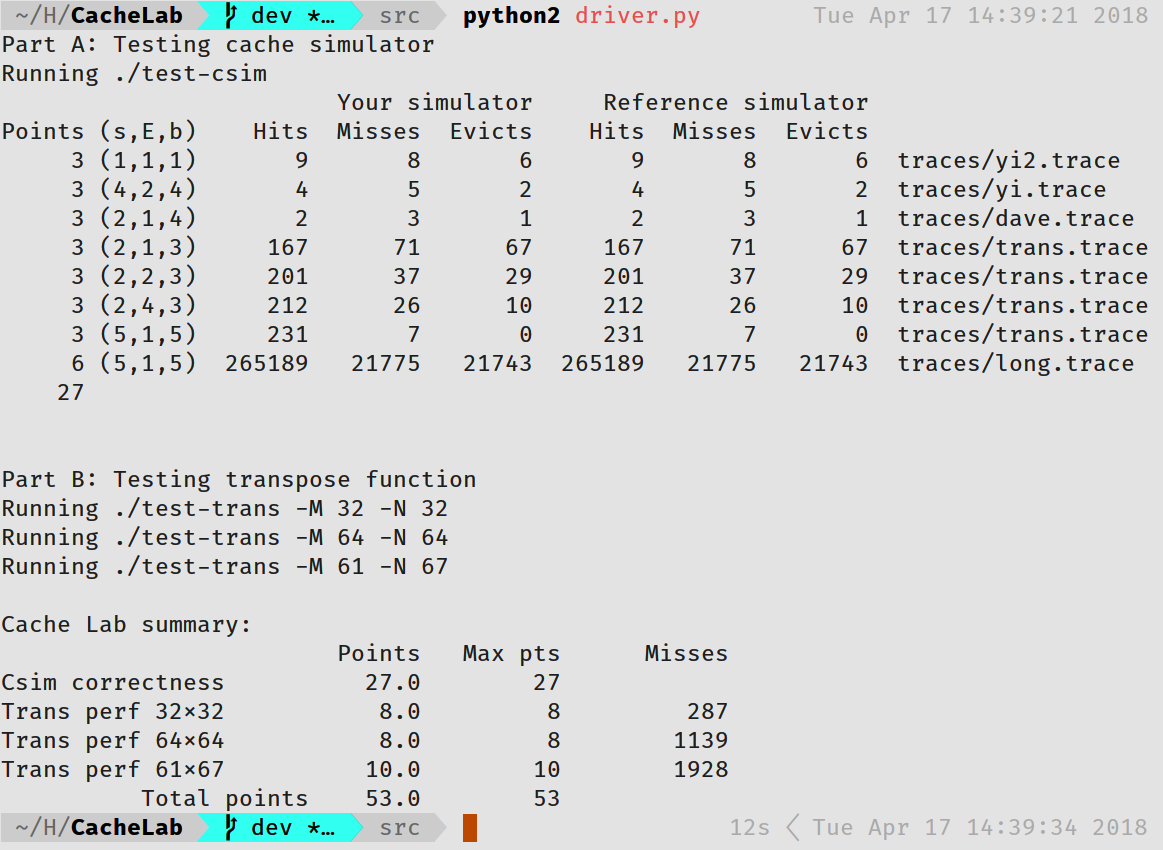
\includegraphics[width=0.9\linewidth]{resultFinal.png}
    \caption{最终测试结果}
    \label{fig:resultFinal}
\end{figure}


